%\documentclass[conference]{IEEEtran}
%\IEEEoverridecommandlockouts
%\documentclass[sigconf]{acmart}
%\let\Bbbk\relax %% fix bug
\documentclass[twocolumn,10pt]{article}
\usepackage[utf8]{inputenc}

% =======================
\usepackage{amssymb}
\usepackage{amsmath}
\usepackage{amstext}
\usepackage{amsopn}
%\usepackage{algorithmic}
\usepackage{graphicx}
\usepackage{textcomp}
\usepackage{xcolor}

\usepackage{textcomp}

\usepackage{boxedminipage}
\usepackage{enumerate}
\usepackage{multirow}
\usepackage{url}
\usepackage{times}
\usepackage{version}
% \usepackage[pdftex]{graphicx}
\usepackage{graphicx} 
\usepackage{epsfig}
\usepackage{epsf}
%\usepackage{graphics}
\usepackage{caption}
\usepackage{subfigure}
\usepackage{algorithm}
\usepackage{algpseudocode}
%\PassOptionsToPackage{bookmarks={false}}{hyperref}
%%%%%%%%%%%%
\usepackage{comment}
\usepackage{multicol}
\usepackage{booktabs}
\usepackage{dblfloatfix}
% ==========================
%\usepackage[a4paper, margin = 2.5cm]{geometry}

\AtBeginDocument{%
  \providecommand\BibTeX{{%
    \normalfont B\kern-0.5em{\scshape i\kern-0.25em b}\kern-0.8em\TeX}}}

\begin{document}

\title{The Accuracy of KNN, decision tree, random forest, SVM, neural network, naive Bayes classifier and PLA for early Prediction of Diabetes}

\author{Hsieh Cheng-Han, Hsu Ting Hao, Sun Shih Yu}
\date{April 2023}
\maketitle

\section*{Abstract}
  This work compares the accuracy of some classifiers for early the prediction of diabetes. More specifically, 
  the research compares the accuracy of k-nearest neighbors (KNN) algorithm, decision tree, random forest, 
  support vector machine (SVM), neural network, naive Bayes classifier, and perceptron learning algorithm (PLA) on the prediction of diabetes, which 
  the dataset is collected with eight features, times of pregnancy, concentration of glucose in blood, blood 
  pressure, skin thickness,  concentration of insulin in blood, body mass index (BMI), the value of diabetes 
  pedigree function and age.

  The result show that XXX is the most accurate on the prediction of diabetes.

\section{Introduction}
\label{sec:Introduction}
  Diabetes is a chronic disease which may cause many complications. There're lots of reason that can put a person 
  at the highly risk of having diabetes, such as age, obesity, lack of exercies, and more on. So many reasons 
  interweave together making the manual prediction on diabetes is nearly impossible. However, lots of works \cite{MUJUMDAR2019292} \cite{MAHBOOBALAM2019100204} \cite{10.3389/fgene.2018.00515}
  show that it is possible to have high accuracy by using machine learning techniques, such as random forest, 
  K-means clustering, neural network, and so on. 

  By collecting the essential data of human body, prediction of diabetes can be turn into classification problem. 
  Imagine that an individual case with essential data is a point in hyperspace, if it is closer to the cluster
  having diabetes, this case is more likely to have diabetes in the future, otherwise, this case is more likely 
  healthy. But there are lots of machine learning techniques born to solve classification problem, it remains a 
  problem that which technique having the hightest accuracy on the prediction of diabetes. 

  To find out which techniques is more suitable to predict diabetes, this work examines the diagnosis of diabetes 
  using KNN algorithm, decision tree, random forest, SVM, neural network naive Bayes classifier, and PLA.
\section{Related works}
\label{sec:Related works}

  \bf{k-nearest neighbors (KNN) classification algorithm}: \rm{The} KNN classification algorithm is a supervised learning 
  method which is first developed by Fix and Hodges \cite{10.2307/1403797}. The idea of KNN is based on the idiom, 
  "birds of a feather flock together". By picking the $k$-nearest neighbors of a data point, the unkonwn class label 
  can be determined. Lots of works \cite{6528591} \cite{8276012} \cite{vijayan2014study} show the fact that KNN performs  
  well for prediction of diabetes disease.

  \bf{decision tree}: \rm{Unlike} KNN uses distance to determine the outcome, 
  decision tree uses a sequence of deicsion that maximize the information gain, which can distinguish the class label of 
  data as much as possible, to determine the outcome. Many works \cite{5893838} \cite{8342938} have applied deicsion tree 
  method and gain a good accuracy. The advantage of decision tree is fast, easy to implement, and the decision is clear. 
  But the disadvantage is that it is very likely over-fitting and the structure of tree will become more complex with the 
  more the class labels. To solve this problem, the following techniques is developed:

  \bf{random forst}: \rm{Instead} of a signle decision tree, random forest use lots of decision trees, which form a "forest". 
  The decision trees are constructed by random subset of dataset. The key differs random forest from decision tree is that 
  while decision trees consider all the possible feature splits, random forests only select a subset of those features, which 
  reduce the risk of overfitting, bias, and overall variance. In \cite{7972337} \cite{10.1007/978-981-16-2164-2_19}, random 
  forest shows that it can greatly reduce the problem of over-fitting of the single decision tree, and gain an ever higher accuracy.

  \bf{support vector machine (SVM)}: \rm{Given} a set of training datas, where each data is labeled as a binary class, such as 
  $0$ and $1$, SVM training algorithm creates a model that assigns new examples to the binay labels by making it a non-probabilistic 
  binary linear classifier. In addition, accroding to \cite{amari1999improving} \cite{hofmann2006support}, SVM can also use a 
  method called kernel trick to effectively perform non-linear classification by implicitly mapping its inputs into a high-dimensional 
  feature space.

  \bf{perceptron learning algorithm (PLA)}: \rm{Perceptron} learning algorithm \cite{gallant1990perceptron} is proposed by Gallant 
  in 1990, which is a fast and simple classification algorithm. However, the limitation of perceptron learning algorithm is that it 
  can only address the data which is linear separable. Thus, the following model connecting layers of perceptrons is proposed:

  \bf{neural network}: \rm{Neural} network have been used in many fields to deal with intricate datas.With input layer, hidden 
  layer and output layer constructed by neurons, each data in dataset is processed while passing through neurons, layer by layer. 
  After the processing, the outcome can be used to predict.Using back propogation, the accuracy of predictions increase in each 
  training. In order to construct the hidden layer more efficient, NAS(Neural Arcitecture Searching) is used to search suitable 
  structure for hidden layer, increasing the accuracy.According to \cite{Gadekallu2020}\cite{Beghriche2021}, many neural network 
  have been constructed and trained already, with high efficiency and accuracy in prediction of diabetes.

  \bf{naive Bayes classifier}: \rm{naive Bayes classifier} as its name suggest, is a machine learning method base on Bayesian 
  theorem, this model will statistic each data and find all conditional probability of each event occurring if each outcome holds. 
  And finally when it is asked to predict the result, the model will evaluate the data which requist provide and find the most 
  likely outcome according to the conditional probability it just recorded. 

\section{KNN}
  \rm{The} rough process of KNN algorithm is described as follow: suppose that there is a dataset which contain $N$ data point, denoted as 
  $(X_i,Y_i)$ where $X_i$ is the features of the i-th individuals data and $Y_i$ is the class label of it. Now 
  a data with unknown class label is given, denoted $(X, Y)$. By a preset distance function $d(P, Q)$, ordering the dataset 
  as $(X_{(1)}, Y_{(1)}), (X_{(2)}, Y_{(2)}), \cdots, (X_{(N)}, Y_{(N)})$ where $d(X_{(1)}, X)\leq d(X_{(2)}, X)\leq\cdots\leq d(X_{(N)}, X)$. 
  Pick the $k$-first class labels to determine the unknow class label, $Y$.

  The algorithm to find $k$ nearest neighbors is the soul of KNN algorithm. The naive way to do that is brute force. By calculating every 
  distance between the dataset and the undetermined data, the desired class can be easily obtained. The time complexity of brute force is $O(n)$. 
  Another way to find $k$ nearest neighbors is approximate nearest neighbors oh yeah (ANNOY). This approximate algorithm is used at Spotify 
  for music recommendations. 
  \begin{figure*}[htb]
    \centering
    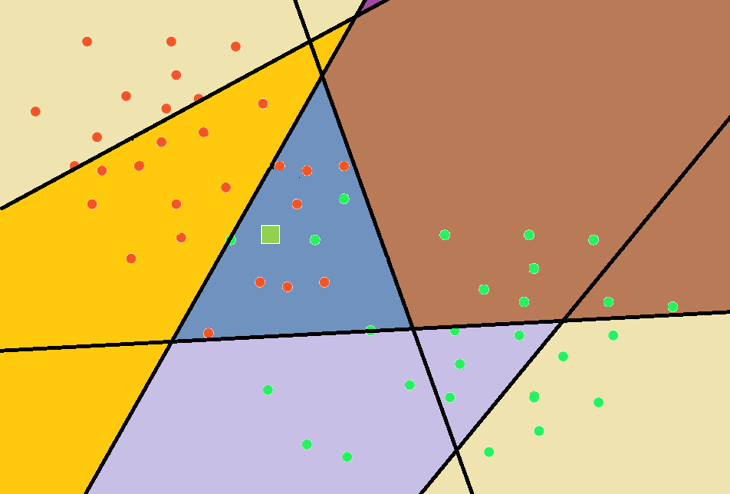
\includegraphics[scale=0.5]{assets/ANNOY-split.png}
    \caption{The region split by ANNOY.}
    \label{fig:ANNOY_split}
  \end{figure*}

  \begin{figure*}[htb]
    \centering
    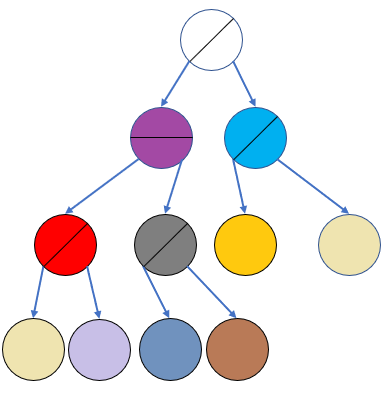
\includegraphics[scale=0.5]{assets/ANNOY-tree.png}
    \caption{The tree structure used by ANNOY.}
    \label{fig:ANNOY_tree}
  \end{figure*}
  Fig. \ref{fig:ANNOY_split} and Fig. \ref{fig:ANNOY_tree} give illustrations of how ANNOY works. The process of ANNOY is detailed as follow: In every iteration, two points are randomly chosen, denoted $\vec x_1,\vec x_2$, 
  and the hyperplane in the middle, whose equation is $\vec n^T\vec x=(\vec x_1-\vec x_2)^T\vec x=(\vec x_1-\vec x_2)^T(\vec x_1+\vec x_2)/2=b$ 
  separates all the points in dataset into two kind, "below" ($\vec n^T\vec x<b$) or "above" ($\vec n^T\vec x>b$). Also, in every iteration, a 
  binary tree structure is constructed whose left child contains all the points "below" the hyperplane and right child contains all the points "above". 
  The end condition is when a side of hyperplane contains points no more than $M$, which is a preset parameter. 
  When query a $k$ nearest neighbors of a point, recursively determine if the point "below" or "above" the hyperplane until reaching the leaf node. 
  The time complexity of construction is $O(n)$, and the time complexity of query is $O(\log n)$.
  But since the region searched may have less $k$ points, the search path shall cover both nodes if the point is too close to the hyperplane. This 
  techniques though may increase the search time, still, it can greatly increase the accuracy of searching.

\section{decision tree}
  Consider a dataset, $D$, which contains $N$ data and class label, the construction of a decision tree can be described as 
  below: suppose there are $M$ candidate decisions, denoted $f_i$. A decision can separate dataset $D$ into $m$ kinds, denote 
  $D'_j$. The decision tree will adopt $\arg\max_{f} G(D, f)=I(D)-\sum^m_{j=1}\frac{N'_j}{N}I(D'_j)$ as node decision, 
  and then recursively construct the tree until the data in separated dataset have the same class label. 
  When a data with unknown class label comes, a decision tree determines recursively by the decision node until the leaf node.
  The function of calculating information, $I$, can be various from implementation. The most famous two information function is 
  entropy, and gini impurity. The formula of information entropy is 
  \begin{equation}
    I_H(X)=-\sum_{x}p(x)\log_2p(x) 
  \end{equation}
  and gini impurity is 
  \begin{equation}
    I_G(X)=1-\sum_{x}p(x)^2
  \end{equation}

\section{random forest}
  Given the fact that a signle decision tree can be easily over-fitting, a technique called "random forest" is developed. By 
  constructing $m$ decision trees with randomized subsets of training dataset, the different decision trees forms a "forest". 
  The process that random forest determine a data with unknown class label can be outlined as follow: suppose for a coming data, 
  $c_i$ decision trees in a random forest classify it as class $i$. Then the random forest will classify the data as class $\arg\max c_i$.

\section{SVM-GA}
  Given a dataset $D$ containing $N$ data points and a label with a binary class label of $0$ or $1$ representing the presence 
  or absence of diabetes, respectively. Individually project each data point in the dataset $D$ onto the hyperplane, we can obtain 
  a point $(X_{i1}, X_{i2}, ..., X_{ij}, ..., X_{in})$, where $X_{in}$ is the i-th individual data of $D$ and  j-th feature of $N$. 
  After obtaining these points, these points are projected onto a hyperplane in $N+1$ dimensions to avoid situations where the 
  data is non-linearly separable. 
  In this case, using the kernel function below as the projection function for each data points in $D$ is a method of reducing 
  the occurrence of non-linear separability: 
	$$\begin{bmatrix}x_1^{(2)} \\x_2^{(2)} \\... \\x_n^{(2)} \\ (\prod_{i=0}^{n} x_i)^{\frac{2}{n}} \end{bmatrix}$$
  After this step, we can find a $N+1$ dimensions hyperplane $w$ that can separate the binary class labels of $0$ and $1$ for 
  the data points. With this hyperplane trained on the training data, we can extend it to classify future data points that do 
  not have binary class labels. 
  Based on \cite{santhanam2015application}, we can use genetic algorithm (GA) to achieve finding better hyperplanes. The following are the 
  steps to find the hyperplane using a GA: Firstly, decide the level of generations ($l$), population size ($n$), 
  variant ($v$), function constant ($b$), elite save rate ($p_e$), and mutations rate ($p_m$). Next, randomly select $N+1$ parameters 
  of floating number between $0$ and $1$ in $w$, repeat it until $n$ hyperplanes are created. 
  In the second step, use $w^t \cdot x - b$ \cite{kumari2013classification} to compare the binary labels of the training data. If 
  $w^t \cdot x - b > 0$, the output is $1$; if $w^t \cdot x - b < 0$, the output is $0$. This determines the accuracy of the $n$ hyperplanes. 
  Then, select the top $n \cdot p_e$ hyperplanes with high accuracy for crossover. The method is to take $v$ feature values from 
  the parent chromosomes to replace or average (randomly) $v$ feature values from the mother chromosomes to create a new hyperplane. 
  During the process, there is a probability of $p_m$ for random mutation of a feature value into a random floating number between 
  $0$ and $1$. After mating $n-n \cdot p_e$ hyperplanes, return this step until the $l$th operation is completed and the best hyperplane 
  is found.
   
\section{PLA}
  Assume that in a dataset $D$, there are two class labels. A perceptron will determine a data point with unknown class label by formula 
  \begin{equation}
    \rm{sign}(w^Tx)
  \end{equation}
  where $w$ is 

\section{neural network}
  Given a dataset $D$ containing $N$ data points and a label with $0$ or $1$ representing the patient is diagnosed with diabetes or 
  not, we need to construct a model with $N$-neurons input layer and 2-neurons output layer.Before we construct the model, we have 
  to find the structure of the hidden layer with NAS.
  We set the number of the layer to 10, with each layer has more than 16 and less than 256 neurons.Define the search space $\mathcal{F}$, 
  which including all the arrays including 10 numbers and each of the number in the array represents the number of neurons in each layers, 
  which is more then 16 and less than 256, like above.We are aiming to find the approximate solution 
  $f= \{x_1, x_2, ..., x_{10}|16\leq x_i \leq 256, 1\leq i \leq 10\}$ $\in$ $\mathcal{F}$, which increase the accuracy of the model in 
  the short term.With simulating annealing algorithm\cite{17235}, we can find the approximate solutions.First, set the initial temperature 
  $T$, the end temperature $T_E$, temperature decreasing rate $R_T$, and a random solution $f^*$.Second, create a model based on the 
  parameter in the $f^*$, and train with $D$.We use cross entropy loss as loss function and Adam as optimization function.After training, 
  we get the average loss of every epoch, $L^*$.Then, start the iteration by swap two of the parameters in $f^*$, get a new array $f^{**}$, 
  train it with dataset, and get its average loss, $L^{**}$.After getting $L^*$ and $L^{**}$, we calculating the difference 
  $\Delta L = L^{**} - L^*$.If $\Delta L \leq 0$, we update $f^* = f^{**}$.Otherwise, we use $e^{\frac{\Delta L}{T}}$ as the probability 
  of the $f^{**}$ accepted as the new solution, get a random number $R^*$ $\in$ [1, 0] from random number generator, if $R^*$ is less than 
  $e^{\frac{\Delta L}{T}}$, we update $f^* = f^{**}$.Then repeat the iteration, but replace the swapping with changing one of the number 
  in $f^*$ to $n, 16 \leq n \leq 256$.
  \begin{equation}
	  f^* = 
	  \begin{cases}
	  f^{**},  &\Delta L\le 0 \\
	  f^{**},  &\Delta L \ge 0 \text{ and } R^*<e^{\frac{\Delta L}{T}} \\ 
	  f^{*},   &\text{else}\\
	  \end{cases}
  \end{equation} 

  After the end of the iteration, multiply $T$ by $R_T$ and continue the iteration until the $T \le T_E$.Then, we get the approximate 
  solution$f=f^*$.Every 2 iteration, the $T$ decreases and lower the probability of $f^{**}$ accepted as the solution.Stimulating annealing 
  can avoid solution stuck at local minimum.Use neural network found by NAS, we can now predict with untrained data with $80\%$ or so accuracy.

\section{Naive Bayes classifier-GA}
  Consider a dataset, $D$, which contain $M$ data points with $k$ class labels. The probability that a random data points belongs to 
  $i$-th class is $P(C_k\mid \bf{x})$ where $C_k$ is the event that data points $\bf{x}=(x_1,\cdots,x_n)$ belongs to $k$-th class.
  By using Bayes' theorem, the probability can be rewritten as 
  \begin{equation}
    \label{eqn:bayes}
    P(C_k\mid x)=\frac{P(C_k)P(\bf{x}\mid C_k)}{P(\bf{x})}
  \end{equation}
  In partice, 
  there is interest only in the numerator of that fraction, because the denominator does not depend on $C_k$ and the values of the 
  features that are given, so the denominator is effectively constant. 
  Then, by chain rule of conditional probability, the numerator of Eq. \ref{eqn:bayes} can be rewritten as
  \begin{equation}
    \label{eqn:rebayes}
    \begin{split}
      &P(C)P(x_1\mid C_k)P(x_2,\cdots,x_n\mid C_k,x_1)
      \\&=\cdots
      \\&=P(C)P(x_1\mid C_k)\cdots P(x_n\mid C_k,x_1,\cdots,x_{n-1})
    \end{split}
  \end{equation}

  Now assume that all features in $\bf{x}$ is mutually independent, $P(x_i\mid x_j, C_k)$ will be equal to $P(x_i\mid C_k)$. 
  Thus, the probability is 
  \begin{equation}
    \label{eqn:prob_classifier}
    P(C_k\mid x)=\frac{P(C_k)\prod^n_{i=1}P(x_i\mid C_k)}{Z}
  \end{equation}
  where $Z$ is a constant. 
  With Eq. \ref{eqn:prob_classifier}, a data points with unknown class label can be classified by choosing the most possible class: 
  \begin{equation}
    \label{eqn:classifier}
    \arg\max_k P(C_k)\prod^n_{i=1}P(x_i=x'_i\mid C_k)
  \end{equation}

  The problem is, when given is a continuous value instead of individual events, it need to be partitioned accroding to specific value 
  which below this value is an individual event while above is other evnet. However, the difficulty is how to find the best partition 
  that can fit the model best. By using gene alogrithm, the answer can be easily found. First, record maximum and minimum values of 
  given data in each dimension. Second, randomly partition data in each dimension according the maximum and minimum value recorded before 
  and repeat 100 times to generate enoguh species. Third, testing the accuracy of the model on the training data and keep top $K$ 
  good species and kill the rest. Then, let the these elites prodece offsprings, which means pass their partitions to offsprings. 
  When there is enough offsprings, all offsprings are going to have mutation, the partitions may slightly shift, 
  merge, split, disappear, or keep originally. Finally, repeat the whole iteration until found the partition that is close to optimal 
  solution after $T$ iterations.

\section{Experiment result}
  This work compare the common classification algorithms, including KNN (with brute force, ANNOY-DFS, ANNOY-BFS), decision tree, 
  random forest, SVM (modified by GA), Neural Network, Naive Bayes classifier (modified by GA), PLA-pocket algorithm. 
  The programming language of KNN, decision tree, random forest and SVM-GA are C++20. And Neural Network, Naive Bayes classifier-GA 
  and PLA-pocket are using Python3 with pytorch and scikit-learn library. 
  Table \ref{table:overall} compares all datasets, which show that ...
  \begin{table*}[htb]
    %\normalsize
    %\centering
    \newcommand{\z}{\phantom{0}}
    \caption{\textsc{Comparison of Classification Techniques.}}
      \vspace{-\baselineskip}
    \begin{tabular}{@{}lccccccl@{}}\toprule
    Technique & Search (s) & testA & testA-normalized & testB & testB-normalized \\ \midrule
    KNN-Brute-Force  & $0.009$ & $76.6169 \pm \z{0}$                & $80.597 \pm 0$               & $78 \pm \z{0}$                 & $80 \pm \z{0}$\\
    KNN-ANNOY-DFS    & $0.003$ & $75.2438 \pm \z{1.8762}$           & $76.1294 \pm 2.0977$         & $74.9 \pm \z{2.5554}$          & $76.4 \pm \z{2.5377}$\\
    KNN-ANNOY-BFS    & $0.012$ & $76.6567 \pm \z{0.5340}$           & $80.597 \pm 0$               & $78.16 \pm \z{0.7310}$         & $80 \pm \z{0}$\\
    decision tree    & $0.009$ & $74.1294 \pm \z{0}$                & $74.1294 \pm 0$              & $76 \pm \z{0}$                 & $77 \pm \z{0}$\\
    random forest    & $0.004$ & $78.6965 \pm \z{1.751}$            & $78.5373 \pm 1.452$          & $77.98 \pm \z{2.083}$          & $77.5 \pm \z{2.516}$\\
    SVM-GA           & $X$ & $X \pm \z{X}$                          & $X \pm X$                    & $X \pm \z{X}$                  & $X \pm \z{X}$\\
    Neural Network   & $3.2$   & $81.7910 \pm \z{2.0294}$           & $80.2985 \pm 1.4106$         & $78 \pm \z{1.6733}$            & $77.5 \pm \z{1.892}$\\
    Naive Bayes classifier-GA    & $X$ & $X \pm \z{X}$              & $X \pm X$                    & $X \pm \z{X}$                  & $X \pm \z{X}$\\
    PLA-pocket       & $X$ & $X \pm \z{X}$                          & $X \pm X$                    & $X \pm \z{X}$                  & $X \pm \z{X}$\\ \midrule
    %&& Search (s) & test & Search(s) & test & Search(s) & test \\ \midrule
    \end{tabular}
    \label{table:overall}
      \vspace{-\baselineskip}
  \end{table*}

\section{Conclusion}
  The experiment result shows that ...
\bibliographystyle{IEEEtran}
\bibliography{main}
\end{document}

